\documentclass[12pt,a4paper]{article}
\usepackage[utf8]{inputenc}
\usepackage[T1]{fontenc}
\usepackage{graphicx}
\usepackage{charter} % Font scelto per il documento
\usepackage{microtype}  % Migliora la qualità tipografica
\usepackage{titling}    % Per personalizzare il titolo
\usepackage[a4paper, margin=2cm]{geometry} % Imposta i margini
\usepackage{setspace} % Per gestire l'interlinea
\setstretch{1.1}  % interlinea di 1.1
\usepackage{enumitem}
\setlist{nolistsep} % Rimuove lo spazio tra gli elementi della lista
\usepackage{float} % Da inserire nel preambolo
\usepackage{wrapfig} % Pacchetto per posizionare testo e immagine affiancati
\usepackage{subfig} % Pacchetto per affiancare immagini
\renewcommand{\thefigure}{\arabic{figure}}
%\setcounter{figure}{6}
\usepackage[hidelinks]{hyperref}  % 'hidelinks' rimuove i bordi rossi
\usepackage{booktabs} % Per migliorare la qualità della tabella
\usepackage{array}    % Per una migliore gestione delle colonne

\usepackage[most]{tcolorbox}
\usepackage{listings}
\usepackage{xcolor}
\usepackage[utf8]{inputenc}


% Rimuovi numeri di pagina sulla prima pagina
\thispagestyle{empty}

% Personalizza titolo (vuoto per ora, lo ricreeremo manualmente)
\title{}
\author{}
\date{}

\begin{document}

    % Creo la copertina manualmente
    \begin{titlepage}
        \begin{center}
            {\Large {UNIVERSITÀ DEGLI STUDI DI SASSARI}}

            \vspace*{\fill}

            {\large Progetto di fine corso:}

            \vspace{1cm}

            {\Large \textbf{PRESENTAZIONE DELLA BASE DATI "OwlBreak"}}
            \vspace{0.3cm}
            \begin{figure}[ht]
                \centering
                
\includegraphics[width=0.4\textwidth]{figures/logo.pdf}       
                \label{fig:logo}
            \end{figure}
     
            \vspace*{\fill}

            \begin{tabular}{l@{\hspace{2cm}}l}
                Studente: & Matricola: \\
                Daniele Picciau & 50056771 \\
                Monica Manai & 50057077
            \end{tabular}

            \vspace{2cm}

            {\large ANNO ACCADEMICO 2024-2025}
        \end{center}
    \end{titlepage}

    \section*{\hspace{15cm}Indice}
    \hrulefill
    \renewcommand{\contentsname}{} % Rimuove completamente il titolo
    \tableofcontents
    \newpage

    % Introduzione
    \section{Analisi dei requisiti}
    \subsection{Descrizione del sistema informativo}
    Si vuole realizzare una base dati per la gestione del bar di una scuola secondaria (di primo o secondo grado) per il quale si vogliono rappresentare:
    \begin{itemize}[leftmargin=1em]
        \item I \textit{Clienti}, che siano essi studenti o personale scolastico, i quali possono effettuare \textit{Ordini} verso gli \textit{Operatori} del bar;
        \item Gli \textit{Ordini} effettuati dai \textit{Clienti};
        \item I \textit{Prodotti} disponibili per essere ordinati dai \textit{Clienti};
        \item Gli \textit{Ingredienti} necessari per la composizione di un \textit{Prodotto};
        \item Gli \textit{Operatori} del bar, i quali si occuperanno di gestire gli ordini dei \textit{Clienti} e di effetuare a loro volta delle richieste di \textit{Rifornimento}
        \item I \textit{Rifornimenti} richiesti dagli \textit{Operatori} per l'acquisto degli \textit{Ingredienti};
        \item I \textit{Fornitori} che possono visionare le richieste di \textit{Rifornimento} degli \textit{Operatori}.
    \end{itemize}

    \vspace{8pt}
    \noindent
    Per i \textit{Clienti}, identificati dall'email istituzionale, si vuole memorizzare il nome e il cognome. Nel caso in cui il cliente sia uno Studente, il sistema registrerà anche la classe di appartenenza. Se, invece, il cliente appartiene al Personale scolastico, verranno archiviati ulteriori dettagli, tra cui il ruolo ricoperto all'interno dell'istituto e il luogo di consegna predefinito degli ordini. Questa distinzione si rende necessaria poiché i membri del personale scolastico, non avendo una postazione fissa all'interno della scuola, devono poter specificare un punto di consegna per ricevere gli ordini in modo più efficiente.\\
    Inoltre, tra i ruoli del personale scolastico, gli unici utenti con privilegi amministrativi aggiuntivi sono gli addetti alla segreteria, che hanno la facoltà di creare, eliminare e modificare gli account dei clienti, siano essi studenti o membri del personale scolastico.

    \vspace{8pt}
    \noindent
    Gli \textit{Ordini} sono identificati dall'email istituzionale del cliente che ha effettuato l'ordine, dal nome del prodotto ordinato, dalla data e dall'ora in cui l'ordine è stato effettuato. Inoltre si vuole memorizzare l'avvenuta consegna dell'ordine da parte degli operatori.
    
    \vspace{8pt}
    \noindent
    Per i \textit{Prodotti}, identificati dal loro nome, si vuole memorizzare il prezzo e un indicatore di disponibilità. Quest'ultimo segnala se almeno uno degli ingredienti necessari alla preparazione del prodotto non è più disponibile, rendendolo temporaneamente non vendibile.

    \vspace{8pt}
    \noindent
    Per gli \textit{Ingredienti},  identificati dal loro nome, si vuole memorizzare una quantità, che indica il numero di unità disponibili, e l'elenco degli allergeni eventualmente contenuti.

    \vspace{8pt}
    \noindent
    Per gli \textit{Operatori}, identificati da un codice ID, si vuole memorizzare la propria email, il nome, il cognome e il ruolo ricoperto all'interno del bar.\\
    Esistono diversi ruoli, ognuno con privilegi specifici, ma tutti gli operatori hanno la possibilità di visualizzare gli ordini effettuati dai clienti:
    \begin{itemize}[leftmargin=1em]
        \item Titolare: è l'unico operatore con la facoltà di aggiungere ed eliminare i dipendenti, oltre a disporre di tutti i permessi riservati agli altri ruoli;
        \item Addetti alle consegne: oltre al titolare, sono gli unici operatori autorizzati a confermare l'avvenuta consegna di un ordine;
        \item Addetti alle vendite: oltre al titolare, sono gli unici operatori abilitati a effettuare e visualizzare le richieste di rifornimento verso i fornitori, nonché a confermarne l'avvenuta consegna. Sono anche responsabili della vendita al bancone e della preparazione degli ordini.
    \end{itemize}

    \vspace{8pt}
    \noindent
    Per i \textit{Rifornimenti}, identificati da un codice ID, si vuole memorizzare l'ingrediente richiesto, la quantità ordinata, la data e l'ora dell'ordine, nonché l'avvenuta consegna da parte dei fornitori.

    \vspace{8pt}
    \noindent
    Per i \textit{Fornitori}, identificati da un codice ID, si vuole memorizzare il nome dell'azienda fornitrice, il nome del titolare e un indirizzo email di riferimento per eventuali comunicazioni o risoluzione di problematiche.

    \subsection{Glossario dei termini}
    \begin{table}[h]
        \renewcommand{\arraystretch}{1.3} % Per aumentare la spaziatura tra le righe
        \centering
        \begin{tabular}{|m{3cm}|m{6cm}|m{3cm}|m{3cm}|}
            \hline
            \textbf{Termine} & \textbf{Descrizione} & \textbf{Sinonimi} & \textbf{Collegamenti} \\
            \hline
            Cliente & Utente con la sola possibilità di effettuare e visualizzare gli ordini. Può essere uno studente o un membro del personale scolastico. & Acquirente & Ordine \\
            \hline
            Ordine & Contiene le caratteristiche dell'ordine effettuato dal Cliente. & Richiesta & Prodotto, Operatore, Cliente \\
            \hline
            Prodotto & Indica un elemento disponibile o non per l'ordinazione. & Articolo & Ingrediente, Ordine \\
            \hline
            Ingrediente & Materia prima utilizzata per la preparazione dei Prodotti. & Componente & Prodotto \\
            \hline
            Operatore & Utente autorizzato alla gestione degli ordini e della vendita. Può effettuare richieste di rifornimento. & Addetto, Venditore & Ordine, Rifornimento \\
            \hline
            Rifornimento & Richiesta di approvvigionamento di Ingredienti ai Fornitori. & Fornitura & Fornitore, Operatore \\
            \hline
            Fornitore & Utente responsabile della fornitura di Ingredienti al sistema, autorizzato alla visualizzazione delle richieste di rifornimento effettuate dagli operatori. & Azienda, Grossista & Rifornimento, Ingrediente \\
            \hline
        \end{tabular}
        \caption{Descrizione dei termini utilizzati nel sistema}
        \label{tab:termini}
        \vspace{-20pt}
    \end{table}

    \subsection{Elenco delle operazioni}
    \subsubsection{Operazioni di inserimento}
    \begin{itemize}[leftmargin=1em]
        \item Inserimento di un nuovo cliente nel sistema;
        \item Inserimento di un nuovo operatore nel sistema;
        \item Inserimento di una nuova richiesta di rifornimento da parte di un operatore verso un fornitore;
        \item Inserimento di un nuovo ordine da parte di un cliente (implica la rimozione della quantità corrispondente di ingredienti dal sistema);
    \end{itemize}

    \subsubsection{Operazioni di modifica}
    \begin{itemize}[leftmargin=1em]
        \item Modifica dei dati di un cliente;
        \item Modifica dei dati di un operatore;
        \item Modifica di una richiesta di rifornimento da parte di un operatore verso un fornitore;
    \end{itemize}

    \subsubsection{Operazioni di eliminazione}
    \begin{itemize}[leftmargin=1em]
        \item Eliminazione di un cliente dal sistema;
        \item Eliminazione di un operatore dal sistema;
        \item Eliminazione di un ordine da parte di un cliente;
        \item Eliminazione di una richiesta di rifornimento da parte di un operatore verso un fornitore;
    \end{itemize}

    \subsubsection{Operazioni di conferma e aggiornamento}
    \begin{itemize}[leftmargin=1em]
        \item Conferma della consegna di un ordine da parte di un operatore;
        \item Conferma della consegna di un rifornimento da parte di un fornitore (implica l'aggiornamento delle scorte di ingredienti, con eventuale inserimento di nuovi ingredienti se necessario);
    \end{itemize}

    \subsubsection{Operazioni di visualizzazione}
    \begin{itemize}[leftmargin=1em]
        \item Visualizzazione degli ordini giornalieri di un singolo cliente;
        \item Visualizzazione della cronologia ordini di un singolo cliente;
        \item Visualizzazione del prezzo totale di un ordine da parte di un cliente;
        \item Visualizzazione dei prodotti disponibili ad essere ordinati.
        \item Visualizzazione, per gli operatori, degli ordini giornalieri suddivisi per luogo di consegna;
        \item Visualizzazione dei dati relativi ai fornitori da parte degli operatori;
        \item Visualizzazione delle richieste di rifornimento da parte degli operatori, raggruppate per fornitore;
        \item Visualizzazione delle richieste di rifornimento da parte dei fornitori, limitata alle richieste a loro indirizzate.
    \end{itemize}

    \newpage
    \section{Modellazione concettuale}
    La modellazione concettuale rappresenta un passaggio fondamentale nella progettazione del sistema, in quanto consente di definire in modo chiaro e strutturato le entità coinvolte e le relazioni tra di esse.\\
    Attraverso l'uso del modello Entità-Relazione (E-R), è possibile ottenere una rappresentazione visiva e formale della logica del database, facilitando l'analisi e la comprensione del dominio applicativo. In questa parte verrà illustrato lo schema E-R del sistema, mettendo in evidenza le principali entità e relazioni. Successivamente, verranno descritte le cardinalità e i vincoli che regolano il funzionamento del sistema.

    \subsection{Schema E-R}
    \begin{figure}[H]
        \centering
        \vspace{-20pt}  % Riduce lo spazio sopra
        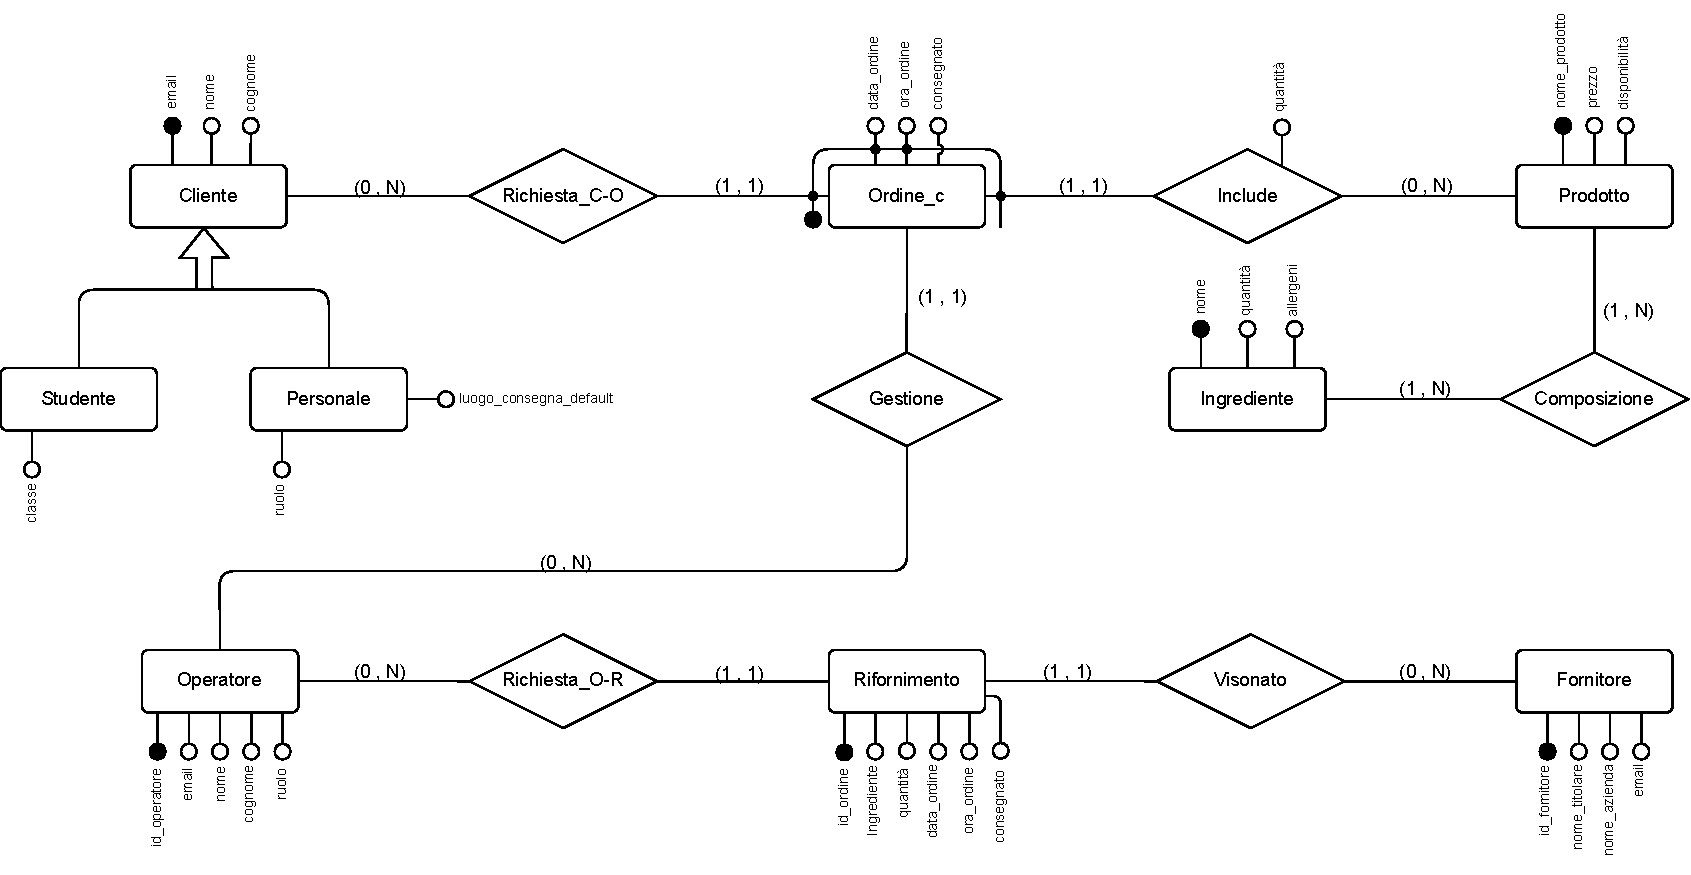
\includegraphics[width=1\textwidth]{figures/Conceptual_model.pdf}
        \vspace{-20pt}  % Riduce lo spazio sopra
        \caption{Modello entità-relazione}
        \label{fig:Conceptual_model}
    \end{figure} 

    \subsection{Descrizione dei vincoli}
    \subsubsection{Cardinalità}
    \begin{itemize}[leftmargin=1em]
        \item \textbf{Richiesta\_C-O} (1:\(N\)): Un cliente può effettuare da 0 a \(N\) ordini, mentre un ordine è effettuato da uno e un solo cliente;
        \item \textbf{Include} (1:\(N\)): Un ordine include uno e un solo prodotto, mentre un prodotto può essere incluso in 0 o \(N\) ordini;
        \item \textbf{Composizione} (\(N\):\(N\)): Un prodotto è composto da 1 o \(N\) ingredienti, mentre un ingrediente può essere parte di 1 o \(N\) prodotti;
        \item \textbf{Gestione} (1:\(N\)): Un ordine è gestito da uno e un solo operatore, mentre un operatore può gestire da 0 a \(N\) ordini;
        \item \textbf{Richiesta\_O-R} (1:\(N\)): Un operatore può effettuare da 0 a \(N\) richieste di rifornimento, mentre una richiesta di rifornimento è effettuata da uno e un solo operatore;
        \item \textbf{Visionato} (1:\(N\)): Un fornitore può visionare da 0 a \(N\) richieste di rifornimento, mentre una richiesta di rifornimento è visionata da uno e un solo fornitore;
    \end{itemize}

    \subsubsection{Regole di vincolo non esprimibili nello schema}
    \begin{enumerate}[leftmargin=3em,label=\textbf{(RV\arabic*)}]
        \item  Gli ordini devono essere effettuati tra le 8 e le 10 del mattino;
        \item La quantità di ogni ingrediente deve essere aggiornata ogni volta che viene effettuato un ordine;
        \item La quantità di ogni ingrediente deve essere aggiornata ogni volta che un rifornimento viene consegnato;
    \end{enumerate}

    \subsubsection{Regole di derivazione}
    \begin{enumerate}[leftmargin=3em,label=\textbf{(RD\arabic*)}]
        \item  Il numero di ordini effettuati da un cliente può essere calcolato contando le istanze della relazione Richiesta\_C-O associate a quel cliente.
    \end{enumerate}






    \newpage
    \section{Modellazione logica}
    Lorem ipsum dolor sit amet, consectetur adipiscing elit. Suspendisse nec ex nec velit mollis rhoncus. Vivamus non magna vulputate magna aliquet feugiat. Vestibulum mi elit, hendrerit quis mollis ut, gravida vel lacus. Morbi quis cursus nulla. Curabitur vitae purus egestas, congue ante nec, malesuada augue. In mollis lectus urna, ac tristique nisi maximus nec. Aenean varius, elit non facilisis facilisis, tellus diam feugiat neque, ut porttitor turpis sapien in ante. Morbi fringilla fermentum ultrices.
    \subsection{Analisi delle ridondanze}
    bla bla bla
    \subsection{Eliminazione delle generalizzazioni}
    bla bla bla
    \subsection{Accorpamento di concetti}
    bla bla bla
    \subsection{Scelta degli identificatori}
    bla bla bla
    \subsection{Modello relazionale}
    bla bla bla
    \subsection{Tavola dei volumi}
    bla bla bla
    \subsection{Tavola delle operazioni}
    bla bla bla

    % Immagine del logo
    \section{Normalizzazione}
    Di seguito è riportato il logo del progetto:
    \subsection{Tecniche di normalizzazione}
    bla bla bla

    % Conclusioni
    \section{Conclusioni}
    In questa sezione finale vengono riassunte le conclusioni del progetto, presentando le implicazioni, i limiti e le direzioni future.

\end{document}